\documentclass[smallextended]{svjour3} 

\usepackage{natbib}

%% Language and font encodings
\usepackage[english]{babel}
\usepackage[utf8x]{inputenc}
\usepackage[T1]{fontenc}

% %% Sets page size and margins
% \usepackage[a4paper,top=3cm,bottom=2cm,left=3cm,right=3cm,marginparwidth=1.75cm]{geometry}

%% Maths
\usepackage{amsmath}
\usepackage{amsfonts}
% \usepackage{amsthm}
\usepackage{amssymb}

%% Useful packages
\usepackage{authblk}
\usepackage{graphicx}
\usepackage{diagbox}
\usepackage[colorlinks=true, allcolors=blue]{hyperref}
\usepackage[colorinlistoftodos,prependcaption,textsize=tiny]{todonotes}
\usepackage[export]{adjustbox}  % http://ctan.org/pkg/adjustbox
\usepackage{siunitx}  % right way to write SI units
\usepackage{booktabs} % define \toprule, ...
\usepackage[linesnumbered,ruled,vlined,]{algorithm2e}
\newcommand\mycommfont[1]{\scriptsize\sffamily{\textit{#1}}}
\SetCommentSty{mycommfont}

%% definitions used in the paper
\newcommand{\xx}{{\bar{x}}}
\newcommand{\yy}{{\bar{y}}}
\newcommand{\eq}{\leftarrow}
\newcommand{\ie}{\emph{i.e.}}
\newcommand{\eg}{\emph{e.g.}}
\newcommand{\dx}{{\bar{x}}}	% data
\newcommand{\dy}{{\bar{y}}}
\newcommand{\dz}{{\bar{z}}}
\newcommand{\tx}{{\dot{x}}}	% solution (tour)
\newcommand{\ty}{{\dot{y}}}
\newcommand{\tz}{{\dot{z}}}
\newcommand{\sx}{{\tilde{x}}}	% solution (sample)
\newcommand{\sy}{{\tilde{y}}}
\newcommand{\sz}{{\tilde{z}}}


\newcommand{\newday}[1]{%
    \section*{#1}%
}


\begin{document}

% \author{}


\title{The Sea Exploration Problem}
\subtitle{Data-driven Orienteering on a Continuous Surface}

\titlerunning{The Sea Exploration Problem}

\author{Jo\~{a}o Pedro Pedroso \and Alpar Vajk Kramer \and Ke Zhang}

\authorrunning{Pedroso \and Kramer \and Zhang}

\institute{J. P. Pedroso  \and A. V. Kramer \at
              INESC TEC and Faculdade de Ci{\^e}ncias, Universidade do Porto, Portugal \\
              % \email{jpp@fc.up.pt, akramer@inesctec.pt}           %  \\
              \email{jpp@fc.up.pt}           %  \\
           \and
           K. Zhang \at
              School of Information Engineering, Wuhan University of Technology, Wuhan, China\\
              \email{kzhang@whut.edu.cn}
}

\date{November 2017}


\maketitle

\begin{abstract}
  This paper describes a problem arising in sea exploration, where the aim is to schedule the expedition of a ship for collecting information about the resources on the seafloor.  The aim is to collect data by probing on a set of carefully chosen locations, so that the information available is optimally enriched.  This problem has similarities with the orienteering problem, where the aim is to plan a time-limited trip for visiting a set of vertices, collecting a prize at each of them, in such a way that the total value collected is maximum.  In our problem, the score at each vertex is associated with an estimation of the level of the resource on the given surface, which is done by regression using Gaussian processes.  Hence, there is a correlation among scores on the selected vertices; this is a first difference with respect to the standard orienteering problem.  The second difference is the location of each vertex, which in our problem is a freely chosen point on a given surface.
\end{abstract}

\keywords{Orienteering, Surface exploration, Gaussian processes, Recognition problems, Tour planning}


\section{Introduction}
\label{sec:introd}

Sea exploration is important for countries with large areas in the ocean under their control, since in the future it may be possible to exploit some of the resources in the seafloor.  However, its contents are largely unknown; for characterizing the seafloor, a preliminary step is to fetch information about its composition.  This is currently being done by sending a ship in an expedition during which an underwater robot, or other equipment, collects samples at selected points.  Such expeditions are typically very costly; additionally, the ship must be available for other commitments at a predetermined port within a rigid and tight time limit.  Nowadays, planning is usually done by experts, based on previously collected information and on intuition.

Even though this paper describes the problem in the context of sea exploration, similar problems arise in other contexts (\eg, fire detection by drones on a forest).  The aim is to schedule the journey of a ship for collecting information about the resources of the seafloor (\eg, composition in certain materials).  The surface being considered here represented as a given (bounded) surface~$S\subset\mathbb{R}^2$.  For the sake of simplicity, we consider that the actual resource level at any point $(x,y) \in S$ can be conveyed by a real number, denoted by~$v(x,y)$.  This \emph{true value} is unknown, except for a limited number $N$ of points in~$S$ for which there is previous empirical information.

Optimal expedition planning involves three subproblems, each corresponding to a different phase on the process.
This first is \textbf{assessment}, which consists of the following: given a finite set of points for which the contents are known, build and indicator function $h(x,y)$ that associates to each point $(x,y) \in S$ the ``attractiveness'' (a real number) for exploring it, in terms of information that can be gathered in case that point is selected for probing.  
The second subproblem is \textbf{planning}, \ie, deciding on the position of a certain number $n$ of points to probe in the next expedition so as to maximize the overall informational reward; the duration of the trip is limited to a known bound. 
The third subproblem, \textbf{estimation}, is related to the final aim of the problem, which is to have an evaluation $w(x,y)$ of the resource level available at any point on the surface~$S$, based on all the information available at the end of the trip.

This paper is organized as follows.  In Section~\ref{sec:litreview} we put this problem in the context of the literature.  Section~\ref{sec:method} describes the method that we developed of tackling the problem; results obtained with it are presented in Section~\ref{sec:results}.  Section~\ref{sec:conclusions} presents some conclusions and future research directions.

\section{Related work}
\label{sec:litreview}

The problem we address in this work is a routing problem with similarities to the \emph{orienteering problem} (OP).  The orienteering problem was initially introduced by \citet{golden1981gtsp}, and its roots are in an outdoor sport with the same name, where there is a set of ``control points'', each with an associated score, in a given area.  Competitors use a compass and a map for assisting in a journey where they visit a subset of control points, starting and ending at given nodes, with the objective of maximizing their total score.  They must reach the end point within a predefined amount of time.

The input to the standard OP consists of a vertex- and edge-weighted graph $G = (V, E)$, a source and a target vertices $s, t \in V$, and a time limit $T$; $V$ is the set of vertices and $E$ is the set of edges.  The goal is to find an $s-t$ walk of total length at most $T$ so as to maximize the sum of weights at vertices visited through the walk.
It can be shown that the OP is NP-hard via a straightforward reduction from the traveling salesman problem.  It is also known to be APX-hard to approximate.  The literature describes an unweighted version (\ie, with a unit score at each vertex), for which a $(2+\epsilon)$ approximation is presented in \citet{Chekuri2012}; for the weighted version, the approximation ratio has a loss with factor $(1 + o(1))$.

An essential difference between the OP and our problem is that in the OP a finite set of vertices is given, from which the solution must be selected.  In our problem, only the surface where some locations may be chosen for sampling is given.  To the best of our knowledge, the closest related work can be found in \citep{Yu2016}. The authors propose a non-linear extension to the orienteering problem (OP), called the \emph{correlated orienteering problem} (COP). They use the COP to model the planning of informative tours for persistent monitoring, through a single or multiple robots, of a spatiotemporal field with time-invariant spatial correlations. The tours are constrained to have a fixed length time budget. Their approach is discrete, as they focus on a quadratic COP formulation that only looks at correlations between neighboring nodes in a network.

Another problem related to ours is \emph{tour recommendation for groups}, introduced in \citet{Anagnostopoulos2017}, where the authors deal with estimating the best tour that a group could perform together in a city, in such a way that the overall utility for whole group is maximized.  They use several measures to estimate this utility, such as the sum of the utilities of members in the group, or the utility of the least satisfied member.  In our case, we estimate this utility (the attractiveness of a point) using a \emph{Gaussian process regression} (see, \eg, \citet{Rasmussen2005}).  This is a generalization of the method known as \emph{kriging}, introduced in \citet{Krige1951} as a geostatistical procedure for generating an estimated surface from a scattered set of points with known values; the original application was on mine valuation.

Gaussian process regression provides estimations for both the mean and the standard deviation; we use the latter as a measure of attractiveness in the assessment phase, and the former as a value the final estimation, after the data set is extended with points actually observed in the expedition.

\section{Method}
\label{sec:method}

\subsection{Assessment and estimation.} The first and the third subproblems, assessment and estimation, are strongly related, in the sense that the aim of the assessment phase is to have a measure of the interest of having empirical information on new points in~$S$ for improving the estimation.  Assessment evaluates how much a given point, if probed, is expected to improve the quality of the estimation done at the third subproblem.

The estimation phase is a regression problem: given the known resource levels at the $N$ previously observed points and at $n$ points to be observed in the expedition, what is the best estimate for the resource level at a new point in~$S$?  A first step for answering this question is to make an assumption on the nature of the underlying function $v(x,y)$.  Our assumption is that is can be conveniently estimated by a Gaussian process.  In this approach, the model attempts to describe the conditional distribution $p(z|(x,y))$ based on a set of empirical observations of $z$ on input $(x,y)$, conveyed as a set of triplets $D = \{(\dz_i,\dx_i,\dy_i)\}_{i=1}^{m}$, where $m$ is the number of samples (in our case, $N$ before the trip and $N+n$ after the trip).   This conditional distribution describes the dependency of the observable $z$ on the input $(x,y) \in S$, assuming that this relation can be decomposed into a systematic and a random component.  The systematic dependency is given by a latent function $w : S \to \mathbb{R}$, which is to be identified based on data $D$.  Hence, the prior is on function values associated with the set of inputs, whose joint distribution is assumed to be multivariate normal.

We use the posteriors inferred thought the Gaussian process model in two ways.  In the assessment phase, we use the standard deviation of the model at each point $(x,y) \in S$ directly as an indicator of attractiveness for probing at that point.  Later, in the estimation phase, the Gaussian process (now with an enlarged data set) is used as a regression for the resource level at any point in~$S$.


\subsection{Planning.} The second subproblem is the selection of points in $S$ for probing, so as to allow a subsequent estimation as accurate as possible.  Points are to be probed in a trip whose maximum duration is known beforehand.  We are thus in the presence of an orienteering problem.  A standard orienteering problem consists of the following: given a graph with edge lengths and a prize that may be collected at each vertex, determine a path of length at most $T$, starting and ending at given vertices, that maximizes the total prize value of the vertices visited.  The problem here is rather particular for several reasons.  The first reason is that besides edge lengths (in our case, edge traversal durations), we have to take into account the time spend in probing at each vertex (which is a parameter of our problem).
The second reason is that the graph may consist of any discrete subset of points $V \subset S$, as long as the duration of the tour --- the time spent on probing and on traveling from a point to the next --- is not larger than the upper bound~$T$.  An additional difficulty is related to the correlation between the prizes obtained in visited vertices; indeed, as the ``prize'' is a measure of the improvement on information obtained by probing, after probing at a given location, probing other locations in this neighborhood are expected to provide less information than distant points (other factors being equal).


\subsection{Tackling the problem}
An instance of this problem must specify the area $S$ being studied, an upper bound~$T$ for the trip duration (including traveling and probing), the duration $t$ required for each probing (here considered independent of the location), and the traveling speed $s$, which allows computing the traveling time between two given points as $d/s$, where $d$ is the Euclidean distance between those points.  Without loss of generality, we are assuming that the initial and end points of the trip to be planned are the same.  Among the instance's data, it must also be provided the previously known data $D = \{(\dz_i,\dx_i,\dy_i)\}_{i=1}^{N}$, corresponding to a set of points $(\dx_i,\dy_i) \in S$ and the corresponding resource level $\dz_i$, for $i=1,\ldots,N$.

In order to evaluate an algorithm for this problem, another set of $K$ points $E = \{(\sx_k,\sy_k)\}_{k=1}^{K}$ at which the level of information predicted by the model is requested, should also be specified.  For these points, the true value of the resource level $v(\sx_k,\sy_k)$ must be known (for computing the error with respect to its estimated value), but it cannot be used by the algorithm.

The main method, making use of a set of auxiliary functions, is provided in Algorithm~\ref{alg:main}.
\begin{algorithm}[!htbp]
  \begin{footnotesize}
    \DontPrintSemicolon
    \SetKwFunction{Orienteering}{Orienteering}
    \SetKwFunction{GPstdev}{GPstdev}
    \SetKwProg{myproc}{procedure}{}{}
    read instance's data $D, T, t, s, S, E$\;
    $a \eq \Orienteering(D, T, t, s, S)$ \;
    update $D$ with probings on all points $a$\;
    $w \eq $ GP regression trained with data $D$\;
    input instance's ``true function'' evaluator $v$\;
    output $\Delta \eq \sum_{(x,y) \in E} {|v(x,y) - w(x,y)|}$\;
  \end{footnotesize}
  \caption{Main procedure.}
  \label{alg:main}
\end{algorithm}

Algorithm~\ref{alg:orienteering} uses the assessment of the attractiveness on a grid of points in~$S$ to determine a trip, \ie, a list of points to visit and probe.  That list is constructed in a greedy way, by determining which is the currently most attractive point, and attempting to add it to the trip.  This is done by checking if a traveling salesman tour including the previous points and the current one can still be done within the time limit (we use an implementation of the algorithm described in \citet{Lin1973} for quickly finding a tour; if its length is feasible, the solution is immediately returned, otherwise the exact model available in \citet{pedroso2012gurobi-book} is used to find the optimal solution with a general-purpose mixed integer programming solver).  After a new point $(x,y)$ is added to the tour, it is conjectured %%% !!!!! find a word better than conjectured !!!
that a simulation using the latest available Gaussian process provides the ``true'' evaluation $z = v(x,y)$, and based on the new speculative datum $(z,x,y)$ the attractiveness allover $S$ is recomputed.
\begin{algorithm}[!htbp]
  \begin{footnotesize}
    \DontPrintSemicolon
    \SetKwFunction{length}{length}
    \KwData{Data: $D = \{(\dz_i,\dx_i,\dy_i)\}_{i=1}^{N}, T, t, s, S$}
    \KwResult{List $a$ of points to visit for probing}
    \SetKwProg{myproc}{procedure}{}{}
    \SetKw{Break}{break}
    \SetKw{Continue}{continue}
    \SetKw{True}{True}
    \SetKw{pop}{pop}
    \SetKw{append}{append}
    \myproc{\Orienteering{$D, T, t, s, S$}}{
      $G \eq \{(x_0+\delta k, y_0+\delta \ell), k=1, \ldots K, \ell=1, \ldots L\}$ \tcp*[f]{grid on $S$} \;
      $a \eq []$ \tcp*[f]{list of points to probe}\;
      \While{\True}{
        $V \eq \GPstdev(D,G)$ \tcp*[f]{points on $G$ sorted by attractiveness} \;
        $(\sigma,x,y) \eq V.\pop()$  \tcp*[f]{remove and return last element of $V$} \;
        $r \eq $ TSP solution visiting $(x,y)$ and all the positions in $a$\;
        \If(\tcp*[f]{including time for probing}){\length(r) < T}
        {
          $a \eq r$
        }
        \Else{\Break}
        $R \eq $ GP regression trained with data $D$\;
        $z \eq R(x,y)$\;
        $D.\append((z,x,y))$\;
      }
      \Return $a$
    }
  \end{footnotesize}
  \caption{Orienteering.}
  \label{alg:orienteering}
\end{algorithm}

Finally, a method for evaluating attractiveness is provided in Algorithm~\ref{alg:attract}.
\begin{algorithm}[!htbp]
  \begin{footnotesize}
    \DontPrintSemicolon
    \SetKwFunction{sort}{sort}
    \KwData{Data: $D = \{(\dz_i,\dx_i,\dy_i)\}_{i=1}^{m}$, grid $\{(,x_i,y_i)\}_{i\in G}$}
    \KwResult{Assessment of standard deviation on grid $G$, $\{(\sigma_i,x_i,y_i)\}_{i\in G}$}
    \SetKwProg{myproc}{procedure}{}{}
    \SetKw{Break}{break}
    \SetKw{Continue}{continue}
    \myproc{\GPstdev{$D, G$}}{
      $R \eq $ GP regression trained with data $D$\;
      $s \eq $ standard deviation function, as evaluated by $R$\;
      $V \eq \{(s(x_i,y_i), x_i, y_i)\}_{i \in G}$ \;
      \sort(V)\;
      \Return V\;
    }
  \end{footnotesize}
  \caption{``Attractiveness'' of points for probing.}
  \label{alg:attract}
\end{algorithm}


\section{Computational results}
\label{sec:results}

\subsection{Benchmark instances used}

In order to assess the quality of the method proposed for solving this problem, we have devised a set of artificial benchmark instances (see Appendix~\ref{sec:instances} for details on their characteristics).

A solution to our problem consisting of two parts: a sequence of locations $a = [(\tx_1,\ty_1), \ldots, (\tx_n,\ty_n)]$ for points where to collect samples (aiming at having maximum information collected), such that the total probing and travel time does not exceed~$T$; and an estimation $\sz_k$ of the level of information predicted by the model on each of the $K$ requested points $E = \{(\sx_k,\sy_k)\}_{k=1}^{K}$.

The evaluation of a method for solving this problem is firstly based on feasibility: the orienteering tour is checked by verifying that the duration of tour $[(\tx_1,\ty_1), \ldots, (\tx_n,\ty_n), (\tx_1,\ty_1)]$ does not exceed~$T$.  Then, the final solution quality is measured by $\sum_{k=1}^{K} {|v(x_k,y_k) - w(x_k,y_k)|}$, as an approximation of $\int \int |v(x,y) - w(x,y)| dx dy$.


\subsection{Results obtained}

Tables~\ref{tab:res16a} to~\ref{tab:res100b} report the results of the computational experiment executed.
Instances for the following cases have been solved: 16 previously known points on a regular grid (Table~\ref{tab:res16a}) and on random positions (Table~\ref{tab:res16b}); 
instances with 49 points on a regular grid (Table~\ref{tab:res49a}) and on random positions (Table~\ref{tab:res49b}); and 
instances with 100 points on a regular grid (Table~\ref{tab:res100a}) and on random positions (Table~\ref{tab:res100b}).
Instances 1 to 5 have an increasing number of local maxima, but are relatively smooth; instances 6 to 10 are less so, with some of them having rather narrow local maxima.
Parameters used in the Gaussian process were roughly tuned using benchmark instances \texttt{f1} to \texttt{f5}; hence, these instances can be seen as the training set, and instances \texttt{f6} to \texttt{f10} as the test set.

In order to have an assessment of the quality of Algorithm~\ref{alg:orienteering}, we compare it to a simple grid search, dividing the time available for exploration into probes on a regular grid, simply avoiding new observations on points for which there was already information available (notice that when the previously available information is very scarce, searching on a grid is a sensible strategy).  Both methods use the same Gaussian process for regression; hence, their initial solution is the same.

As expected, increasing the number of initial points with information available increases the quality of the initial estimation with a Gaussian process; this can be observed in the first column of tables~\ref{tab:res16a} to~\ref{tab:res100b}.  Having those points disposed in a grid is usually preferable, but this is not a general pattern.  The estimation is much improved when new data becomes available (an exception is observed on instance \texttt{f7} with 100 initial points randomly spread, where adding more data on a regular grid strangely decreased the quality of the final estimation; this is likely to be a limitation of the optimizer used for training the Gaussian processes).

The main results are summarized in Table~\ref{tab:results}, where we can observe that the orienteering method proposed in Algorithm~\ref{alg:orienteering} is generally superior to grid search.  This superiority increases with the quantity of initial points available, indicating that, \eg, only 16 points is not enough information for preparing a probing plan based on those data.

\begin{table}[!htbp]
  \centering
  \caption{Summary of results: winning situations for grid search and for our algorithm.}
  \begin{tabular}{lccc}
    Benchmarks & Grid search & Orienteering \\\hline
    16-grid    &      4      &    6      \\
    49-grid    &      2      &    8      \\
    100-grid   &      2      &    8      \\
    16-random  &      6      &    4      \\
    49-random  &      5      &    5      \\
    100-random &      1      &    9      \\
  \end{tabular}
  \label{tab:results}
\end{table}


\begin{table}[!htbp]
  \centering
  \caption{Results for instances with 16 initial points on a regular grid.}
\sisetup{
round-mode = places,
round-precision = 1 }%
\begin{tabular}{r|SSSS}
  \toprule
  {Name} & {Initial} & {Grid} & {Orienteering} \\
  \midrule
  f1  & 37179.778811730626 &    911.7041527629668 & 622.5733146415533   \\ 
  f2  & 40696.71629611851  &   7509.139481896236  & 6094.044365285448   \\ 
  f3  & 52257.19063109544  &   6441.789703795481  & 7935.324447441893   \\ 
  f4  & 60996.87798721852  &   9768.986380976852  & 14253.397340910882  \\ 
  f5  & 61339.81507957516  &   9910.764540742326  & 9415.666057980878   \\ 
  f6  & 56.15433842301819  &      1.3856423092470 & 1.7802725274184277  \\ 
  f7  & 730.0779372614868  &   686.2554885474509  & 675.8285069442941   \\ 
  f8  & 34764.77470303922  &  1415.7205093903674  & 975.096960919084    \\ 
  f9  & 55643.53539494152  &  2116.000166529825   & 2007.9100295870455  \\ 
  f10 & 57428.169869564044 &  4547.918542351984   & 6306.045952962949   \\
  \bottomrule
\end{tabular}
  \label{tab:res16a}
\end{table}

\begin{table}[!htbp]
  \centering
  \caption{Results for instances with 16 initial points on random positions.}
\sisetup{
round-mode = places,
round-precision = 1 }%
\begin{tabular}{r|SSSS}
  \toprule
  {Name} & {Initial} & {Grid} & {Orienteering} \\
  \midrule
  f1  & 45327.99223 & 981.0667238753 & 393.0387719508  \\ 
  f2  & 34509.91816 & 6874.414139594 & 8629.612791418  \\ 
  f3  & 48476.62221 & 7282.731103267 & 11217.08391896  \\ 
  f4  & 40291.26654 & 11324.12807287 & 13683.13276886  \\ 
  f5  & 67108.55182 & 8293.709629573 & 13505.75216142  \\ 
  f6  & 51.22287120 & 1.526349702613 & 1.855124146473  \\ 
  f7  & 710.9913316 & 686.6961762270 & 680.3497195064  \\ 
  f8  & 44127.14824 & 1414.289432736 & 1138.942175462  \\ 
  f9  & 62934.96119 & 2048.881168471 & 5661.822273599  \\ 
  f10 & 39025.07259 & 5966.048960339 & 5711.869140318  \\
  \bottomrule
\end{tabular}
  \label{tab:res16b}
\end{table}



\begin{table}[!htbp]
  \centering
  \caption{Results for instances with 49 initial points on a regular grid.}
\sisetup{
round-mode = places,
round-precision = 1 }%
\begin{tabular}{r|SSSS}
  \toprule
  {Name} & {Initial} & {Grid} & {Orienteering} \\
  \midrule
  f1  & 12108.97137666 & 181.731601068111 & 908.18259137810  \\ 
  f2  & 19311.70659492 & 4443.06488192847 & 4312.2358937250  \\ 
  f3  & 24787.39796680 & 5159.35433327471 & 4698.6601148211  \\ 
  f4  & 24215.69612876 & 5197.24636896981 & 4915.5596035177  \\ 
  f5  & 24157.86703339 & 5358.61322013083 & 5047.5866646386  \\ 
  f6  & 5.086410579774 & 1.28152906355877 & 1.5002020919382  \\ 
  f7  & 2442.656906440 & 1186.07508274749 & 1030.0429129309  \\ 
  f8  & 14703.08318244 & 2304.45314508131 & 1414.8509135940  \\ 
  f9  & 23072.05523854 & 2811.45162635772 & 1993.6269417231  \\ 
  f10 & 25322.55762799 & 5009.43979135893 & 4032.6911555676  \\
  \bottomrule
\end{tabular}
  \label{tab:res49a}
\end{table}

\begin{table}[!htbp]
  \centering
  \caption{Results for instances with 49 initial points on random positions.}
\sisetup{
round-mode = places,
round-precision = 1 }%
\begin{tabular}{r|SSSS}
  \toprule
  {Name} & {Initial} & {Grid} & {Orienteering} \\
  \midrule
  f1  & 13997.25353754 & 480.36351574704 & 733.2685926695  \\ 
  f2  & 17605.45853853 & 3267.8122742294 & 6330.861960372  \\ 
  f3  & 28619.33116749 & 4357.5807145301 & 3726.929905739  \\ 
  f4  & 35975.46408136 & 7740.8285866607 & 6191.163191926  \\ 
  f5  & 45076.35307099 & 9694.1523334896 & 6937.110554097  \\ 
  f6  & 10.44123444584 & 1.2535376537810 & 1.475482027571  \\ 
  f7  & 678.3053485673 & 685.52857459377 & 675.9856747658  \\ 
  f8  & 23555.57918052 & 826.83341088183 & 752.7486088134  \\ 
  f9  & 22699.31402901 & 1893.8774797966 & 2837.814343250  \\ 
  f10 & 18552.67478668 & 3835.0922993059 & 4540.825450144  \\
  \bottomrule
\end{tabular}
  \label{tab:res49b}
\end{table}



\begin{table}[!htbp]
  \centering
  \caption{Results for instances with 100 initial points on a regular grid.}
\sisetup{
round-mode = places,
round-precision = 1 }%
\begin{tabular}{r|SSSS}
  \toprule
  {Name} & {Initial} & {Grid} & {Orienteering} \\
  \midrule
  f1  & 1731.7896272028 & 44.05442596446 & 13.981762013760  \\ 
  f2  & 6426.9197973531 & 3221.388218697 & 2709.2257612550  \\ 
  f3  & 8809.9251941359 & 4060.648972336 & 2801.2783635260  \\ 
  f4  & 11401.920965345 & 5408.026716541 & 4552.7476132560  \\ 
  f5  & 11740.116089340 & 5584.462915850 & 5103.4756775125  \\ 
  f6  & 2.1472886022932 & 1.229213042754 & 1.2623032999025  \\ 
  f7  & 4889.2470181203 & 3015.201113918 & 3714.0467289974  \\ 
  f8  & 10252.211519105 & 5633.021459386 & 4140.5621072140  \\ 
  f9  & 13115.303241305 & 6356.344860132 & 4435.7027588911  \\ 
  f10 & 14806.818020229 & 7249.516893536 & 6028.6725916451  \\
  \bottomrule
\end{tabular}
  \label{tab:res100a}
\end{table}

\begin{table}[!htbp]
  \centering
  \caption{Results for instances with 100 initial points on random positions.}
\sisetup{
round-mode = places,
round-precision = 1 }%
\begin{tabular}{r|SSSS}
  \toprule
  {Name} & {Initial} & {Grid} & {Orienteering} \\
  \midrule
  f1  & 770.81741855039 & 15.0984707795 & 12.4006697730  \\ 
  f2  & 16669.033357815 & 5057.86816844 & 2904.09709395  \\ 
  f3  & 16099.794024674 & 5152.52474174 & 4009.43488407  \\ 
  f4  & 17974.570559110 & 6475.31068938 & 3115.24569124  \\ 
  f5  & 25562.243575807 & 4947.56294429 & 4131.39991938  \\ 
  f6  & 1.5818950001535 & 1.08188582527 & 1.54268838260  \\ 
  f7  & 675.68542582178 & 682.798544398 & 675.419307010  \\ 
  f8  & 883.83751620512 & 6666.55104402 & 2555.98483683  \\ 
  f9  & 3736.2339833565 & 2079.54693306 & 837.336643633  \\ 
  f10 & 9484.1353914149 & 3338.82099048 & 3018.13328387  \\
  \bottomrule
\end{tabular}
  \label{tab:res100b}
\end{table}

In order to visualize the improvements that are obtained by probing, we have prepared figures \ref{fig:f1} and \ref{fig:f5}, each with the true function, the initial estimation (in the cases shown, with 16 points), and with the estimation after probing with the orienteering tour.  As can be seen, the application of our method results in a clear improvement on the approximation of the true function.
\begin{figure}[h!tbp]
  \centering
  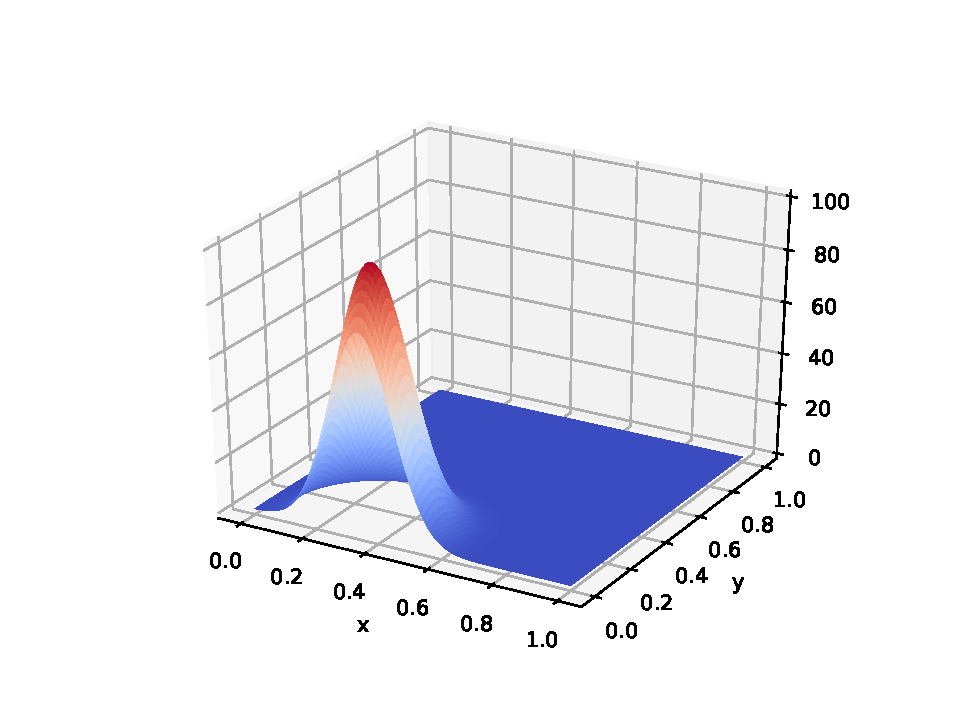
\includegraphics[width=.32\textwidth,trim=100 30 50 50,clip=True]{f1-16-true.pdf}
  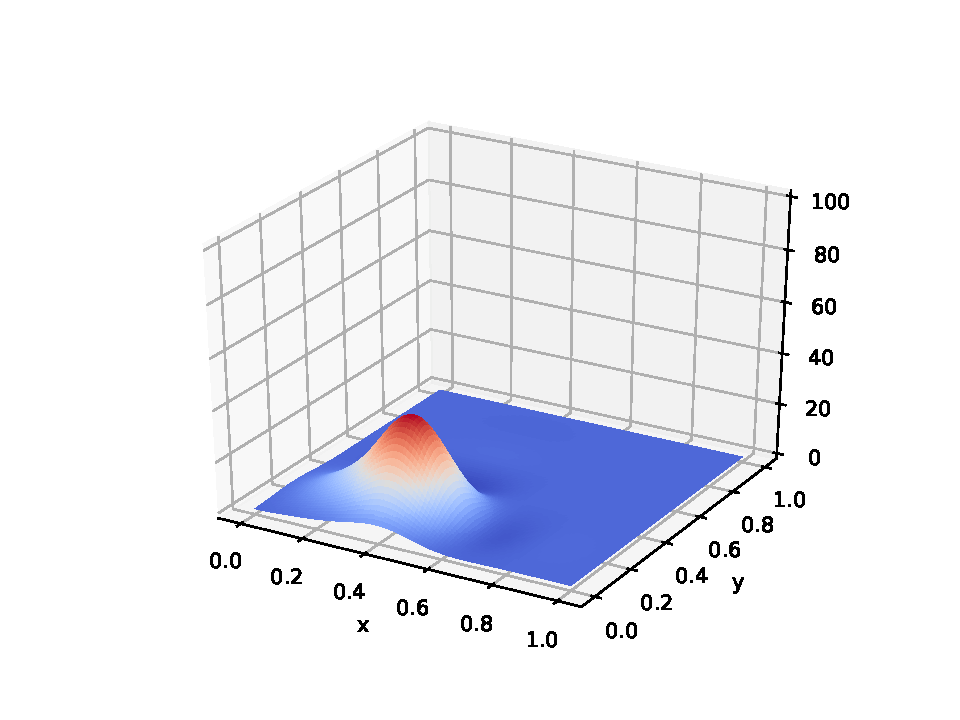
\includegraphics[width=.32\textwidth,trim=100 30 50 50,clip=True]{f1-16-prev.pdf}
  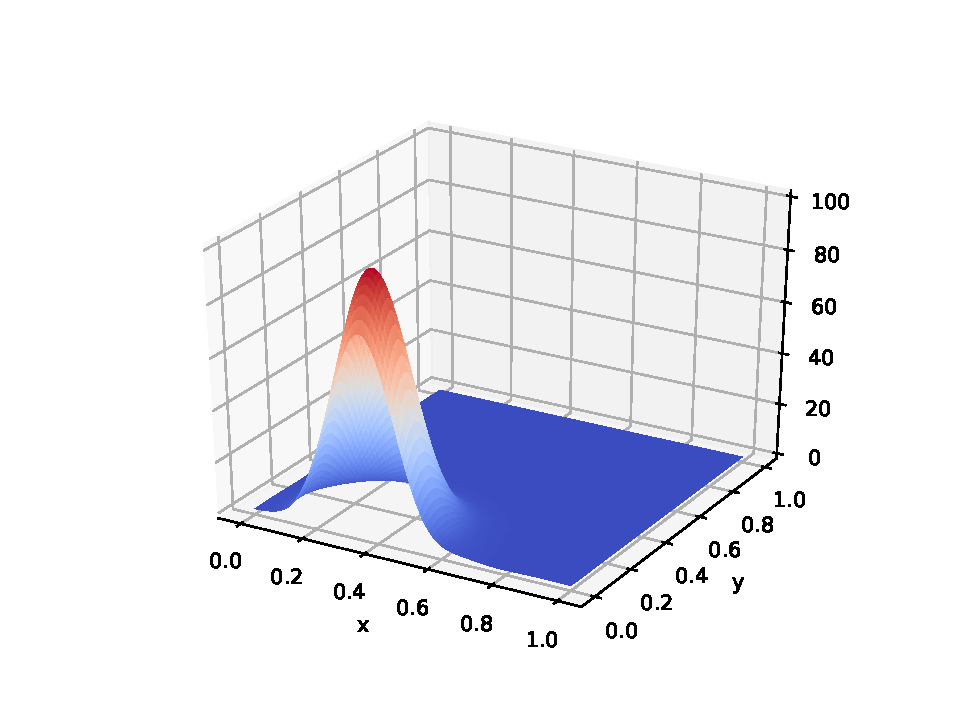
\includegraphics[width=.32\textwidth,trim=100 30 50 50,clip=True]{f1-16-post.pdf}
  \caption{``True'' function used in instance \texttt{f1} (left), initial estimation (center) and estimation after probing (right).}
  \label{fig:f1}
\end{figure}

\begin{figure}[h!tbp]
  \centering
  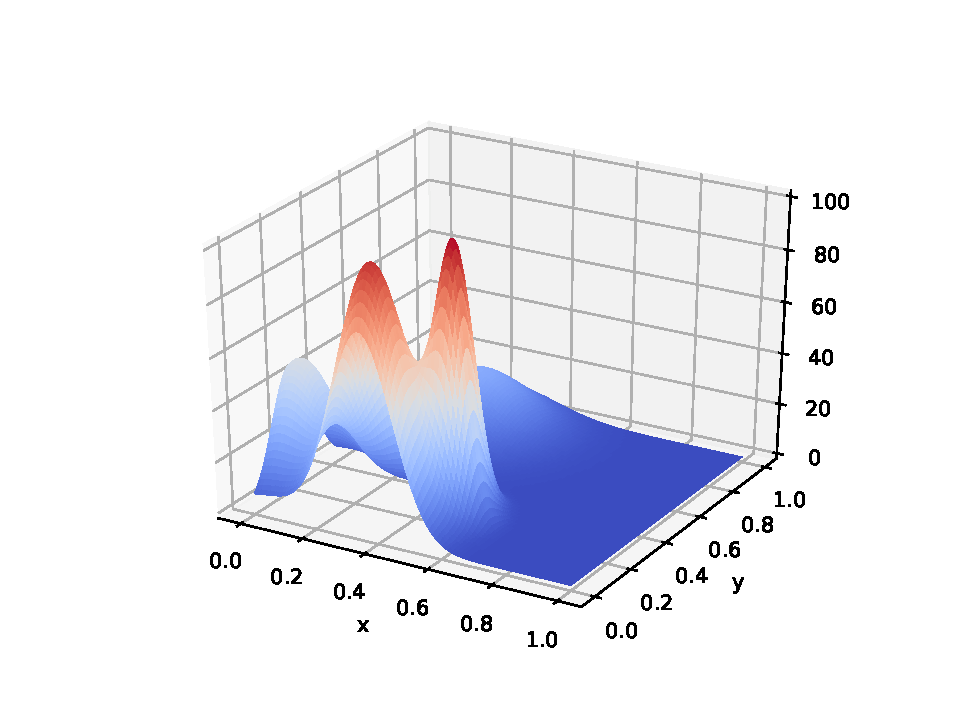
\includegraphics[width=.32\textwidth,trim=100 30 50 50,clip=True]{f5-16-true.pdf}
  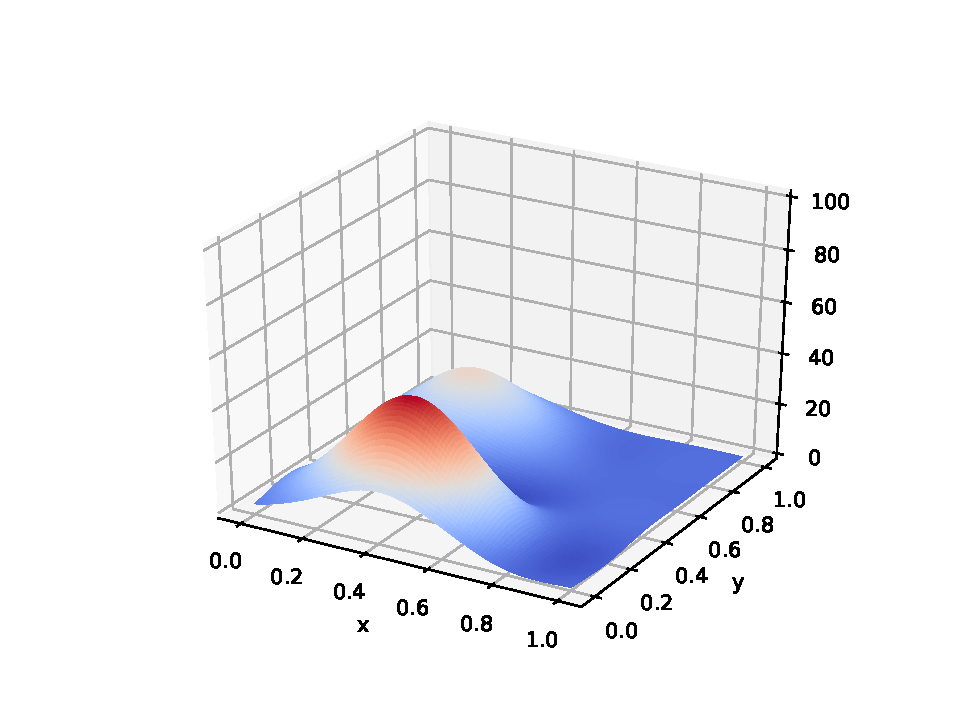
\includegraphics[width=.32\textwidth,trim=100 30 50 50,clip=True]{f5-16-prev.pdf}
  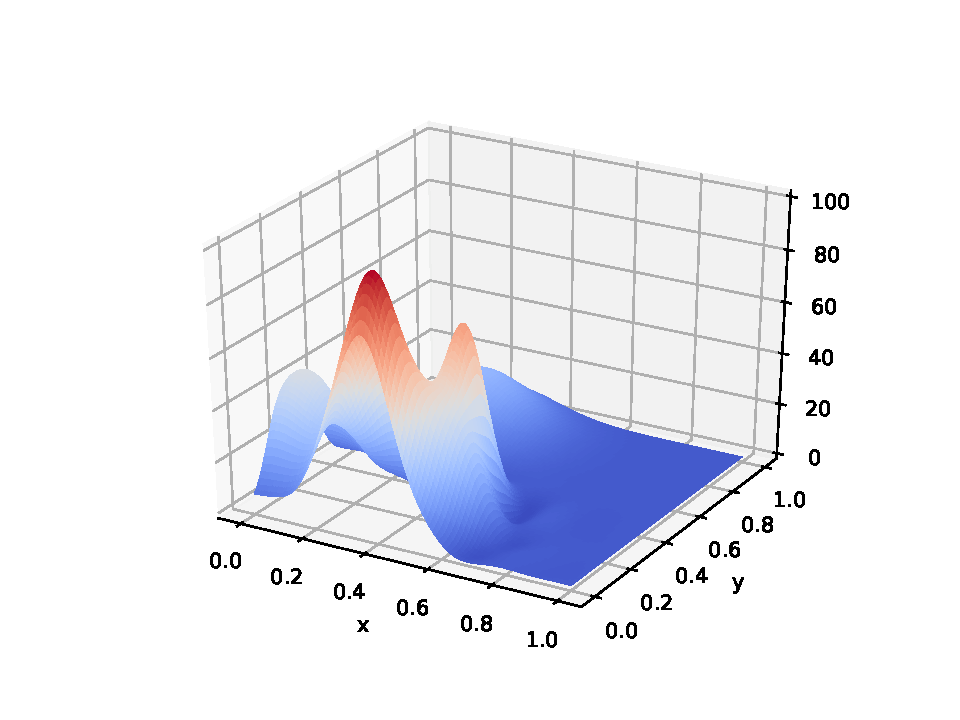
\includegraphics[width=.32\textwidth,trim=100 30 50 50,clip=True]{f5-16-post.pdf}
  \caption{``True'' function used in instance \texttt{f5} (left), initial estimation (center) and estimation after probing (right).}
  \label{fig:f5}
\end{figure}


\section{Conclusions}
\label{sec:conclusions}

This paper describes a problem arising in sea exploration, where the aim is to decide the schedule of a ship expedition for collecting information about the resources of the seafloor.  The setting involves the simultaneous use of tools from machine learning and combinatorial optimization.   We propose a method for its solution, dividing the process in three phases: assessment (building an indicator function that associates to each point in the sea a value for the interest in probing it),
planning (deciding on the position of points to probe in the next trip) and estimation (predicting a value of the resource level at any point on the surface).  The results obtained indicate that using the method here proposed clearly improves the quality of the estimation, by probing at promising points and adding the newly collected information to a regression step, which is based on Gaussian processes.

An interesting direction for future research is adapting the algorithm proposed here in order to deal with real-time changes in the path, reacting in the most appropriate way to information available as new observations arrive.


\begin{acknowledgements}
This work was partially supported by project  "Coral - Sustainable Ocean Exploitation: Tools and Sensors/NORTE-01- 0145-FEDER-000036", financed by the North Portugal Regional Operational Programme (NORTE 2020), under the PORTUGAL 2020 Partnership Agreement, and through the European Regional Development Fund (ERDF).
\end{acknowledgements}

\bibliographystyle{spbasic}
% \bibliographystyle{spphys}
\bibliography{coral}


\appendix

\section{Benchmark instances used}
\label{sec:instances}

A complete description of the benchmark instances used is available at the author's homepage\footnote{\url{http://www.dcc.fc.up.pt/~jpp/code/CORAL}}.
In summary, there are 10 different ``true'' functions that should be guessed, \texttt{f1} to \texttt{f10}; an illustration of their shapes is provided in figures \ref{fig:f1} to~\ref{fig:fB}.

The area $S$ being studied is considered to be $(x,y) \in [0,1] \times [0,1]$.  The set of points initially available are noiseless evaluations of functions \texttt{f1} to \texttt{f10}, either in a regular grid (\eg, as in Table~\ref{tab:f1-16grid}) or randomly spread in $S$ (as in Table~\ref{tab:f1-16rand}).

Other relevant data are: the probing time $t=1$ time units; the speed of traveling $s=1$; and parameter $T=100$.  The starting and ending nodes are located at coordinates (0,0).    

As for the evaluation of the quality of the algorithms, the differences between the true and the predicted values, $w(x,y)$ and $v(x,y)$,  are assessed on $K$ points $E$  on a mesh $x,y \in \{0, 0.01, \ldots, 1\}$.

\begin{table}[!htbp]
  \centering
  \caption{Evaluations of f1 on a grid.}
\begin{tabular}{l|rrrr}
\diagbox{$\bar{x}$}{$\bar{y}$}
      &  0.20 &  0.40 &  0.60 &  0.80\\\hline
  0.2 &  0.00 &  0.02 &  8.21 & 60.65\\
  0.4 &  0.00 &  0.00 &  0.15 &  1.11\\
  0.6 &  0.00 &  0.00 &  0.00 &  0.00\\
  0.8 &  0.00 &  0.00 &  0.00 &  0.00\\
\end{tabular}
  \label{tab:f1-16grid}
\end{table}

\begin{table}[!htbp]
  \centering
  \caption{Evaluations of f1 at random positions.}
  \label{tab:f1-16rand}
  \sisetup{
    round-mode = places,
    round-precision = 3 }%
  \begin{tabular}{SSS}
    {$x$} & {$y$} & {$f(x,y)$} \\\hline
0.0254458609934608	& .5414124727934966	& 0.0 \\ % 7.729637656959195e-06\\
0.029040787574867943	& .22169166627303505	& 0.17910654005215518\\
0.0938595867742349	& .02834747652200631	& 3.338438486158641\\
0.13436424411240122	& .8474337369372327	& 0.0 \\ % 7.646167162951911e-13\\
0.21659939713061338	& .4221165755827173	& 0.084613952016198\\
0.22876222127045265	& .9452706955539223	& 0.0 \\ % 1.1775677447084087e-15\\
0.23308445025757263	& .2308665415409843	& 13.845273128139127\\
0.43788759365057206	& .49581224138185065	& 0.008218117557316357\\
0.4453871940548014	& .7215400323407826	& 0.0 \\ % 4.0994102141623627e-08\\
0.49543508709194095	& .4494910647887381	& 0.027187155905827275\\
0.651592972722763	& .7887233511355132	& 0.0 \\ % 7.058121622918677e-12\\
0.762280082457942	& .0021060533511106927	& 0.016852780725354247\\
0.763774618976614	& .2550690257394217	& 0.003676848494094813\\
0.8357651039198697	& .43276706790505337	& 0.0 \\ % 1.135890188571365e-06\\
0.9014274576114836	& .030589983033553536	& 0.0 \\ % 2.4491571971025315e-05\\
0.9391491627785106	& .38120423768821243	& 0.0 \\ % 2.512057131852312e-08\\
  \end{tabular}
\end{table}

\begin{figure}[!htbp]
  \centering
  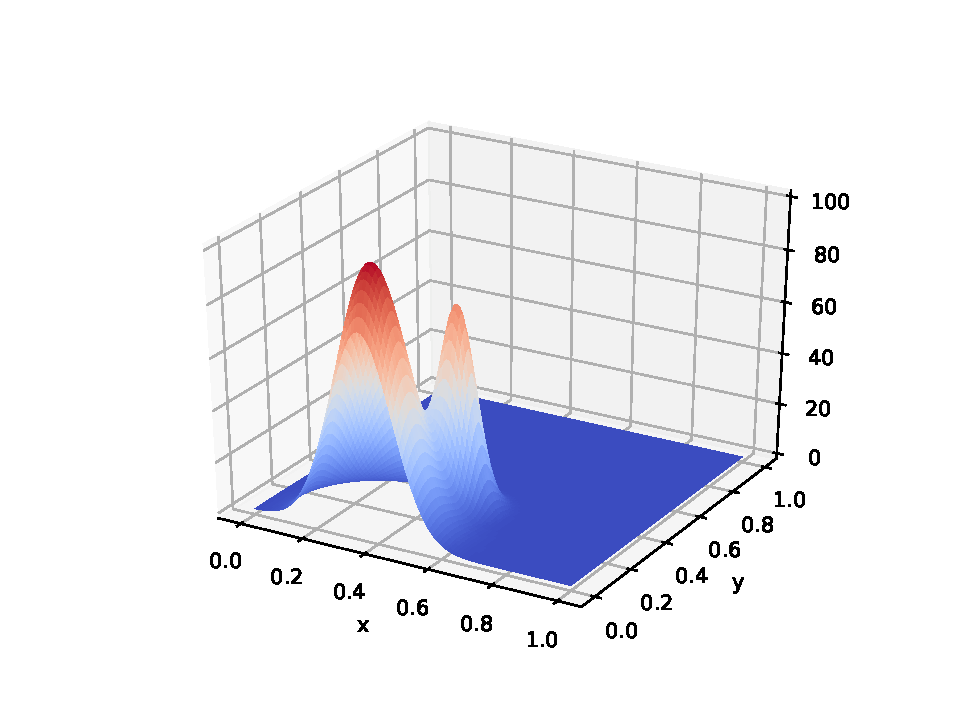
\includegraphics[width=.33\textwidth,trim=100 30 50 50,clip=True]{f2.pdf}
  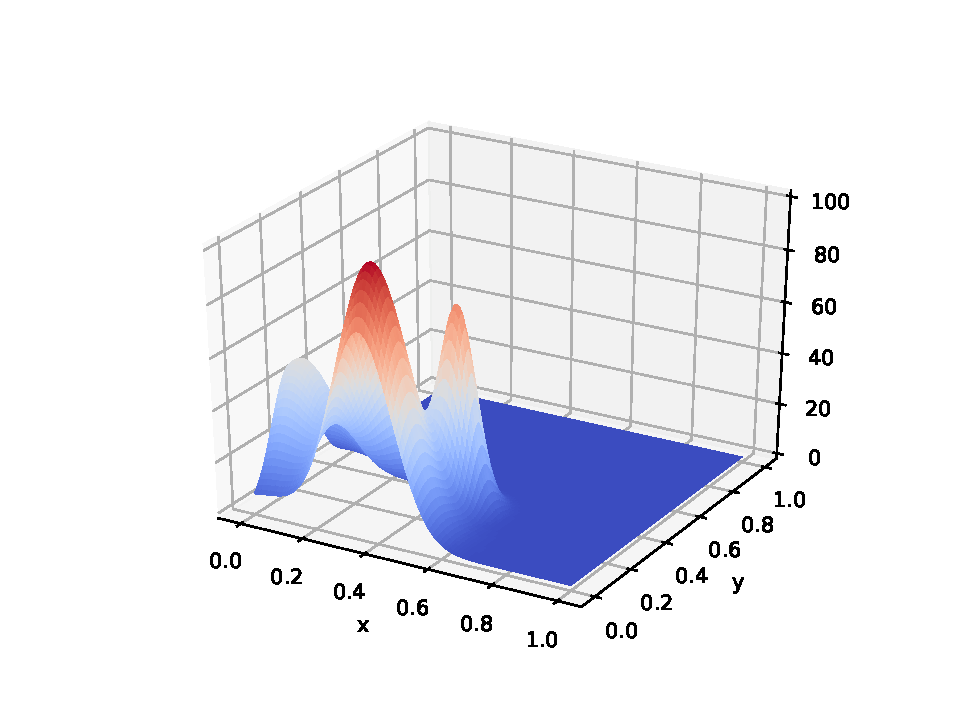
\includegraphics[width=.33\textwidth,trim=100 30 50 50,clip=True]{f3.pdf} 
  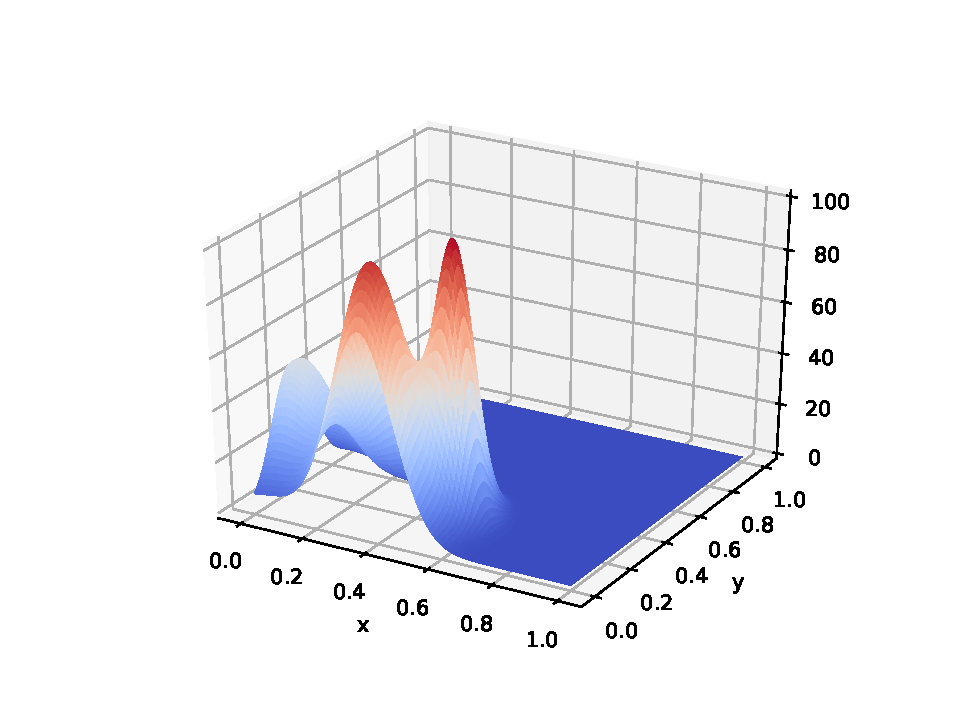
\includegraphics[width=.33\textwidth,trim=100 30 50 50,clip=True]{f4.pdf} 
  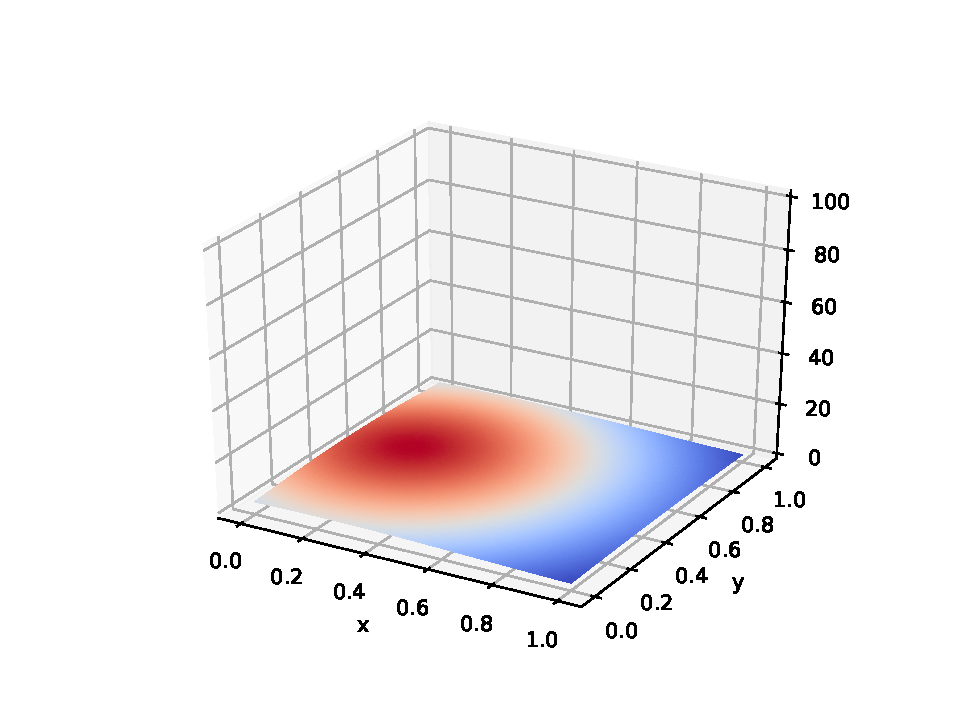
\includegraphics[width=.33\textwidth,trim=100 30 50 50,clip=True]{f6.pdf}
  \caption{``True'' function used in instances \texttt{f2, f3} (top) and \texttt{f4, f6} (bottom).}
  \label{fig:fA}
\end{figure}
 
\begin{figure}[!hbtp]
  \centering
  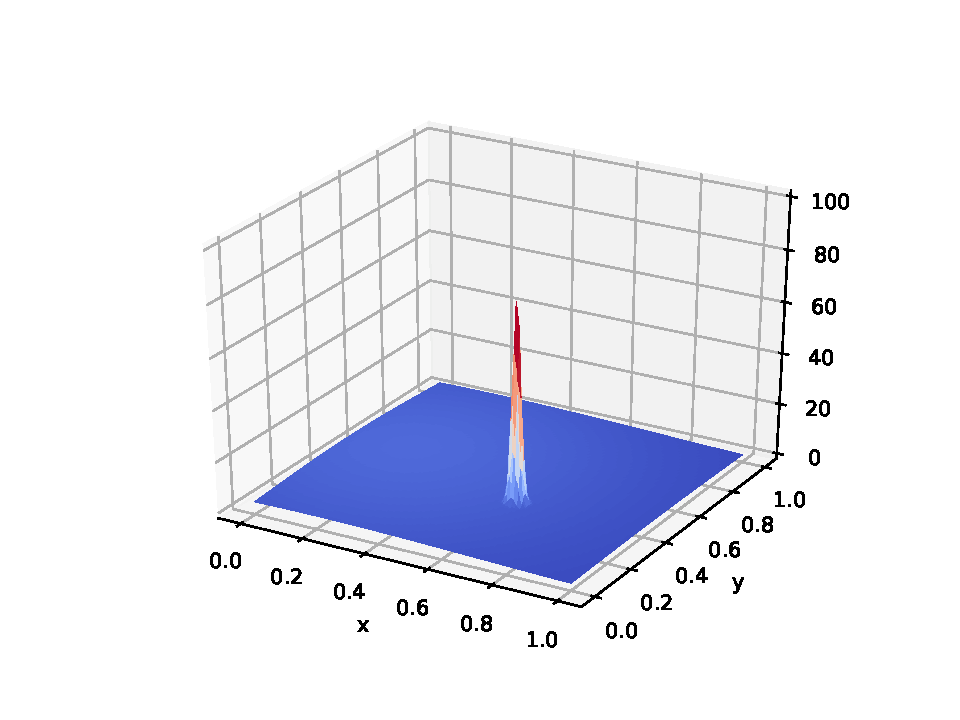
\includegraphics[width=.33\textwidth,trim=100 30 50 50,clip=True]{f7.pdf}
  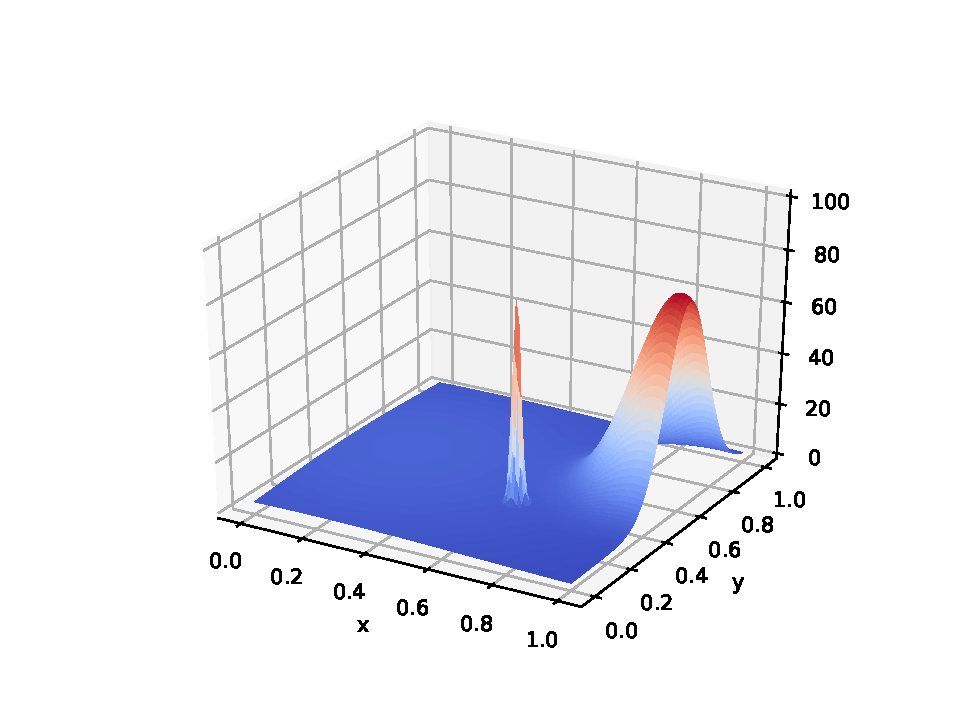
\includegraphics[width=.33\textwidth,trim=100 30 50 50,clip=True]{f8.pdf}
  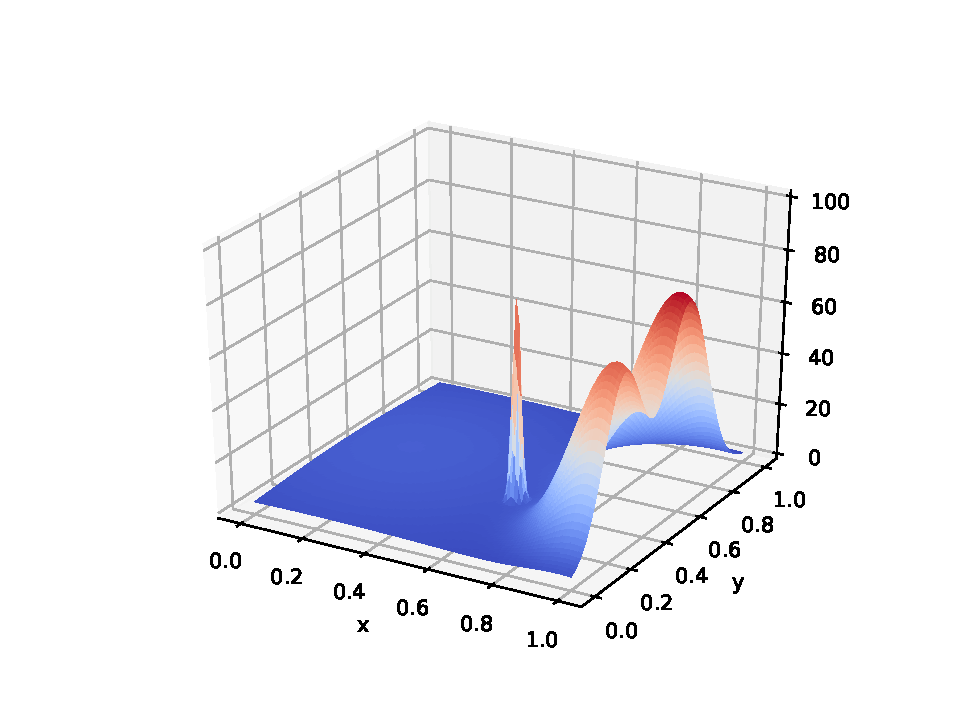
\includegraphics[width=.33\textwidth,trim=100 30 50 50,clip=True]{f9.pdf}
  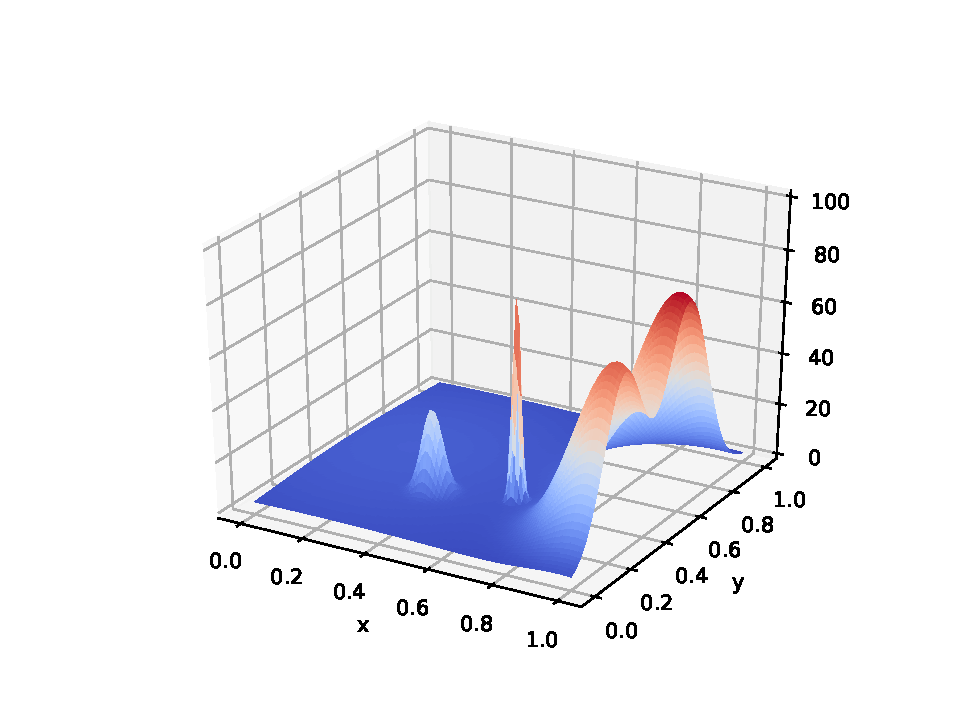
\includegraphics[width=.33\textwidth,trim=100 30 50 50,clip=True]{f10.pdf}
  \caption{``True'' function used in instances \texttt{f7, f8} (top) and \texttt{f9, f10} (bottom).}
  \label{fig:fB}
\end{figure}

\end{document}
